\section{Projektorganisation} \label{section:Projektorganisation}

Der Grund daf�r, dass dieses Projekt ins Leben gerufen wurde, ist das grundlegende Interesse und der Durst nach finanzwirtschaftlichem Wissen, sowie die Projektauftraggeber Professor Mag. Hans Brabenetz und Professor Dr. Helmut Vana. Der Projektleiter ist Peer Nagy und das Team besteht noch zus�tzlich aus zwei weiteren Entwicklern: Gabriel Pawlowsky und Josef Sochovsky.

\begin{figure}[h]
	\centering
		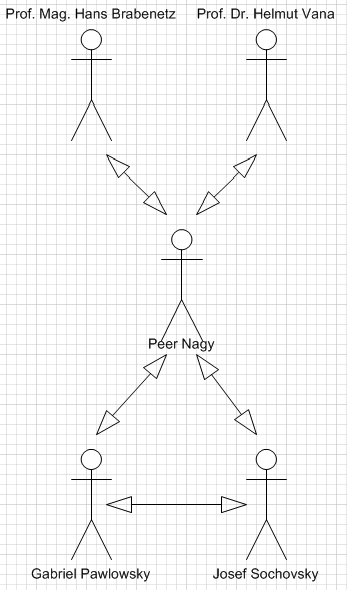
\includegraphics[width=0.60\textwidth]{graphics/wirmachbarkeit/Projektorganisation.PNG}
	\caption{Projektorganisationsdiagramm erstellt mit Microsoft Visio}
	\label{fig:Projektorganisation}
\end{figure}

Die Zust�ndigkeiten der Projektteammitglieder sind folgenderma�en verteilt:

\begin{itemize}
	\item Peer Nagy
		\subitem F�hrendes Projektmanagement
		\subitem Entwicklung des Algorithmus (forschender Teil)
		\subitem Entwicklung der Marktzustandserkennung (forschender Teil)
	\item Gabriel Pawlowsky
	 	\subitem Programmierung der \gls{bts}
	 	\subitem Entwicklung des Algorithmus (forschender Teil)
	 	\subitem Entwicklung der Marktzustandserkennung (forschender Teil)
	\item Josef Sochovsky
		\subitem Entwicklung des Algorithmus (durchf�hrender Teil)
		\subitem Entwicklung der Marktzustandserkennung (durchf�hrender Teil)
\end{itemize}

Das Testing des Erzeugnis wird von dem Team als Gruppe bearbeitet.